% Options for packages loaded elsewhere
\PassOptionsToPackage{unicode}{hyperref}
\PassOptionsToPackage{hyphens}{url}
\PassOptionsToPackage{dvipsnames,svgnames,x11names}{xcolor}
%
\documentclass[
]{article}
\usepackage{amsmath,amssymb}
\usepackage{iftex}
\ifPDFTeX
  \usepackage[T1]{fontenc}
  \usepackage[utf8]{inputenc}
  \usepackage{textcomp} % provide euro and other symbols
\else % if luatex or xetex
  \usepackage{unicode-math} % this also loads fontspec
  \defaultfontfeatures{Scale=MatchLowercase}
  \defaultfontfeatures[\rmfamily]{Ligatures=TeX,Scale=1}
\fi
\usepackage{lmodern}
\ifPDFTeX\else
  % xetex/luatex font selection
\fi
% Use upquote if available, for straight quotes in verbatim environments
\IfFileExists{upquote.sty}{\usepackage{upquote}}{}
\IfFileExists{microtype.sty}{% use microtype if available
  \usepackage[]{microtype}
  \UseMicrotypeSet[protrusion]{basicmath} % disable protrusion for tt fonts
}{}
\makeatletter
\@ifundefined{KOMAClassName}{% if non-KOMA class
  \IfFileExists{parskip.sty}{%
    \usepackage{parskip}
  }{% else
    \setlength{\parindent}{0pt}
    \setlength{\parskip}{6pt plus 2pt minus 1pt}}
}{% if KOMA class
  \KOMAoptions{parskip=half}}
\makeatother
\usepackage{xcolor}
\usepackage{graphicx}
\makeatletter
\def\maxwidth{\ifdim\Gin@nat@width>\linewidth\linewidth\else\Gin@nat@width\fi}
\def\maxheight{\ifdim\Gin@nat@height>\textheight\textheight\else\Gin@nat@height\fi}
\makeatother
% Scale images if necessary, so that they will not overflow the page
% margins by default, and it is still possible to overwrite the defaults
% using explicit options in \includegraphics[width, height, ...]{}
\setkeys{Gin}{width=\maxwidth,height=\maxheight,keepaspectratio}
% Set default figure placement to htbp
\makeatletter
\def\fps@figure{htbp}
\makeatother
\setlength{\emergencystretch}{3em} % prevent overfull lines
\providecommand{\tightlist}{%
  \setlength{\itemsep}{0pt}\setlength{\parskip}{0pt}}
\setcounter{secnumdepth}{-\maxdimen} % remove section numbering
\usepackage{preamble_ai_project}
\usepackage[backend=bibtex,style=numeric]{biblatex}
\bibliography{references}
\ifLuaTeX
  \usepackage{selnolig}  % disable illegal ligatures
\fi
\IfFileExists{bookmark.sty}{\usepackage{bookmark}}{\usepackage{hyperref}}
\IfFileExists{xurl.sty}{\usepackage{xurl}}{} % add URL line breaks if available
\urlstyle{same}
\hypersetup{
  colorlinks=true,
  linkcolor={Blue},
  filecolor={Maroon},
  citecolor={Blue},
  urlcolor={Blue},
  pdfcreator={LaTeX via pandoc}}

\author{}
\date{}

\begin{document}

\intro{}

\hypertarget{introduction}{%
\section{1 -- Introduction}\label{introduction}}

Dans ce document, nous approfondirons des techniques de regression
logistique et ``Naive Bayes'' comme outils d'apprentissage superivisés.

Citation Test: \cite{LinearModels}

\hypertarget{muxe9thodologie}{%
\section{2 -- Méthodologie}\label{muxe9thodologie}}

Pour la suite de ce projet les outils suivants ont été utilisés dans
chaque parties:

\begin{itemize}
\tightlist
\item
  \href{https://www.python.org/}{python}
\item
  \href{https://numpy.org/}{numpy}
\item
  \href{https://scikit-learn.org/stable/}{sklearn}
\item
  \href{https://matplotlib.org/}{matplotlib}
\end{itemize}

\hypertarget{gradient-descent}{%
\subsection{2.1 -- Gradient Descent}\label{gradient-descent}}

Dans cette section, une implémentation de la ``descente en gradient'' a
été réalisée. la fonction a la signature suivante

\begin{lstlisting}
  def gradient_descent(df, params: NDArray, alpha: float, num_iters: int) -> NDArray:  
\end{lstlisting}

Elle calcule de manière itérative le(s) paramètre(s) \code{params} qui
minimisent la fonction dont \texttt{df} est le gradient avec un ``taux
de convergence'' \code{alpha}.

La fonction a été testé avec la fonction \code{scipy.optimize.fmin}
\cite{ScipyOptimizeFmin} de la librairie \texttt{scipy} sur la fonction
suivante: \[
f(x) = x * \cos(\pi  (x + 1))
\]

avec différents \(x_0 \in \{-\pi, 0, \pi\}\) (valeur initiale de
\code{params}, i.e.~\texttt{NDArray} avec D=0).

Les minimas locaux trouvés par les deux fonctions sont les suivants:

\begin{figure}
\centering
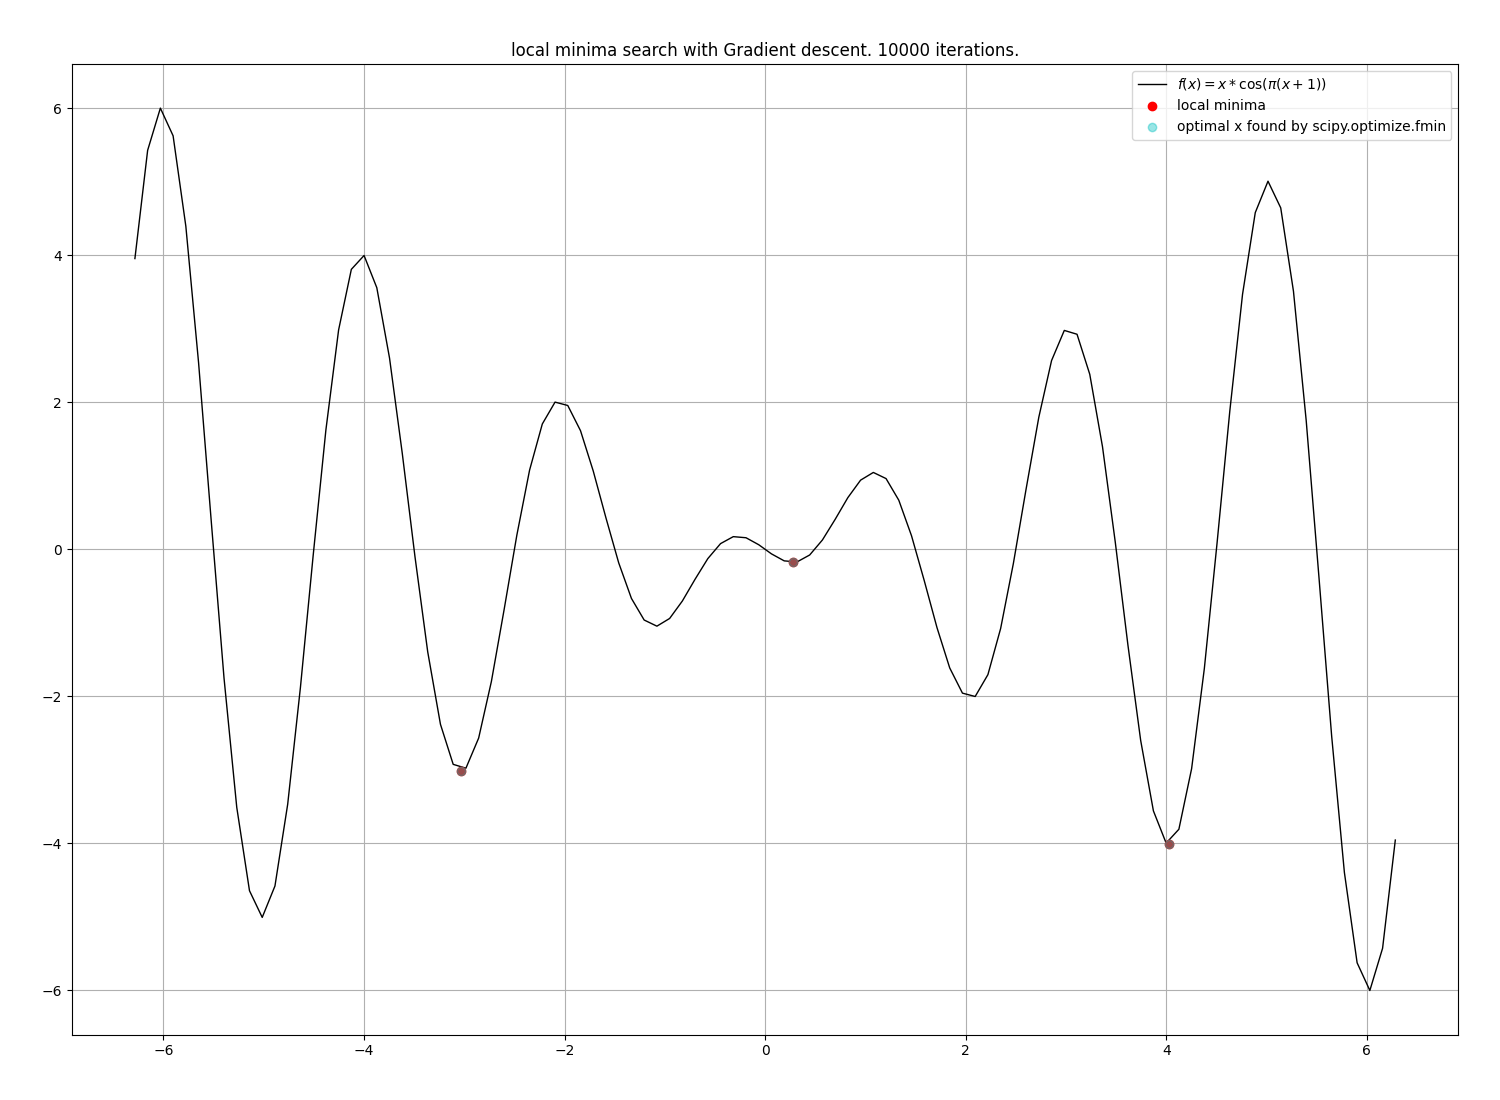
\includegraphics[width=0.71\textwidth,height=\textheight]{../res/3.1_gradient_descent_minima.png}
\caption{minimas locaux\_gradient descent}
\end{figure}

\newpage{}

Ce résultat illustre bien 2 choses: la première est que l'implémentation
de la descente en gradient fonctionne correctement puisque pour chaque
points trouvé par notre fonction est confondu avec celui trouvé par la
fonction de scipy (c'est ce qui donne cette teinte ``grise''). La
deuxième est que la ``qualité'' du minima local (i.e.~la distance avec
le minima globale) dépend fortement de la valeur initiale et ce pour les
deux fonctions.

\hypertarget{ruxe9sultats}{%
\section{3 -- Résultats}\label{ruxe9sultats}}

\printbibliography[heading=bibintoc, title={Références}]

\begin{itemize}
\tightlist
\item
  TODO: ajouter les autres références des documentations utilisées
\end{itemize}

\end{document}
